
  {\bf\large Model 1: A Diagram and A C++ Code Snippet} \\[-15pt]
  \begin{center}
    \small
    \begin{tabular}{p{2in}p{3in}}
      \begin{minipage}{2in}
        \centering\par\vskip 10pt
        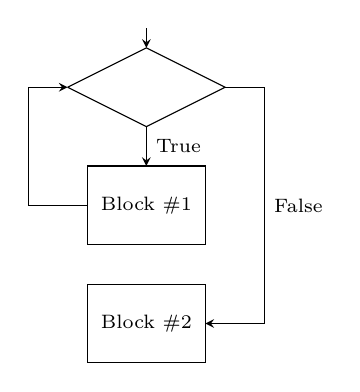
\begin{tikzpicture}
          % two rectangles
          \draw (0.25,1.5) -- (1.75,1.5) -- (1.75,2.5) -- (0.25,2.5) -- (0.25,1.5);
          \draw (0.25,0) -- (1.75,0) -- (1.75,1) -- (0.25,1) -- (0.25,0);
          % one triangle
          \draw (0,3.5) -- (1,3) -- (2,3.5) -- (1,4) -- (0,3.5);
          % five arrows
          \draw[-stealth] (1,4.25) -- (1,4);
          \draw[-stealth] (1,3) -- node[right] {\scriptsize True} (1,2.5);
          \draw[-stealth] (0.25,2) -- (-0.5,2) -- (-0.5,3.5) -- (0,3.5);
          \draw[-stealth] (2,3.5) -- (2.5,3.5) -- node[right] {\scriptsize False} (2.5,0.5) -- (1.75,0.5);
          % text
          \node[] at (1,2) {\scriptsize Block \#1};
          \node[] at (1,0.5) {\scriptsize Block \#2};
        \end{tikzpicture}
        \par\vskip 4pt\ \      
      \end{minipage}
      &
      \begin{minipage}{3in}
        \begin{minted}[
          frame=lines,
          framesep=2mm,
          bgcolor=gray!15,
          baselinestretch=1.2,
          linenos,
	  firstnumber=6
        ]{cpp}
  // print a person's name 10 times        
  string name;
  cout << "Enter your name: ";
  cin >> name;
  int x = 0;
  while (x < 10) {
    cout << name << endl;
    x = x + 1;
  }
  cout << "Nice to meet you!" << endl;
        \end{minted}
      \end{minipage}
    \end{tabular}
  \end{center}
  \TPMargin{5pt}
  
  
  {\it\large Refer to Model 1 above as your team develops consensus answers
    to the questions below.}
    \par\vskip 10pt
    
  \begin{enumerate}
    \itemsep 20pt
    
    \item Which lines of code go with the following shapes on the provided diagram?
      \par\vskip 20pt
      \begin{enumerate}[(a)]
        \itemsep 15pt
        \item The diamond \hfill 
          \fillin[Line 11 contains the condition in the diamond][4in]
        \item The ``Block \#1'' rectangle \hfill 
          \fillin[Lines 12 and 13 make up the statements in block \#1][4in]
        \item The ``Block \#2'' rectangle \hfill 
          \fillin[Line 15 contains the statement in block \#2][4in]
      \end{enumerate}
      
    \item Every loop structure requires three different actions.  Identify the line in the C++
      code snippet above that corresponds to each of these actions.
      \par\vskip 20pt
      \begin{enumerate}[(a)]
        \itemsep 15pt
        \item {\bf Initialize} a variable to control the number of loop iterations. \hfill\fillin[Line 10][1in]
        \item {\bf Test} a condition to determine if we should keep looping. \hfill\fillin[Line 11][1in]
        \item {\bf Update} the variable involved in the test condition. \hfill\fillin[Line 13][1in]
      \end{enumerate}     

\newpage

    \item The complete program is in {\tt activity07a.cpp}.  Run the program and
      answer the following questions.
      \begin{enumerate}[(a)]
        \item What would the model program do differently if line 10 was: \mintinline{cpp}|int x = 1;|?
          \begin{solution}[0.4in]
            It would only print out 9 copies of the name.
          \end{solution}
        \item What would the model program do differently if line 11 was: \mintinline{cpp}|while (x <= 10) {|?
          \begin{solution}[0.4in]          
            It would print out 11 copies of the name.
          \end{solution}
        \item What would the model program do differently if line 13 was: \mintinline{cpp}|x=x+2;|?
          \begin{solution}[0.4in]
            It would only print out 5 copies of the name.
          \end{solution}
      \end{enumerate}
      \par\vskip -40pt\null
      
    \item Change one or more of lines 10, 11, and 13 to make the program print the name 23 times.\key\\[-2.5mm]
      
      \begin{solution}[1.25in]
        \par
        Answers will vary, but one solution is to change line 6 to read:
        \begin{center}
          \mintinline{cpp}| while ( x < 23 ) {|
        \end{center}        
      \end{solution}
      